\chapter{基于深度学习的个性化推荐}
\section{问题定义}
推荐系统的应用场景繁多,被推荐的对象也各式各样,为了便于研究推荐方法,一系列的评测任务被提出,其中最为著名的就是电影评分预测任务。
该任务在数学形式上可以表达为,给定$\mathbf{N}$个用户和$\mathbf{M}$个物品,评分$\mathbf{r}_{ij}$代表第$i$个用户给第$j$个物品的评分数据,
数值的高低对应用户对该物品的兴趣程度。在真实世界的应用场景中,用户通常只会评价一小部分物品(相对于整个物品集合),
因此,这些评分数据构成了一个巨大的稀疏矩阵$\mathbf{R} \in \mathbb{R}^{N \times M}$,推荐系统的目标就是去预测这些缺失的评分数据,
最后我们可以将具有较高预测分的且用户没有观看过的电影推荐给用户。

\begin{figure}[htbp]
\centering
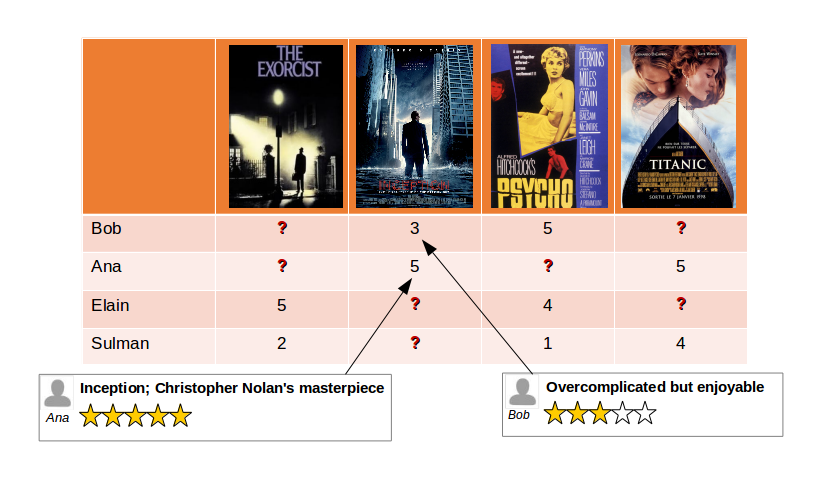
\includegraphics[scale=0.6]{images/task1.png}
\caption{电影评分预测任务样例1}
\label{fig:task1}
\end{figure}

图\ref{fig:task1}给出的电影频分预测任务样例中,存在$4$个用户和$4$部电影,
已经在评分日志中发现的9个评分数据,这些数据构成了一个$4 \times 4$的稀疏评分矩阵,
我们的目标就是构建模型刻画用户之间的关系、物品之间的关系和用户物品之间的关系,
去预测图中问号表示的缺失评分数据,并根绝这些预测评分进行电影推荐。

\begin{figure}[htbp]
\centering
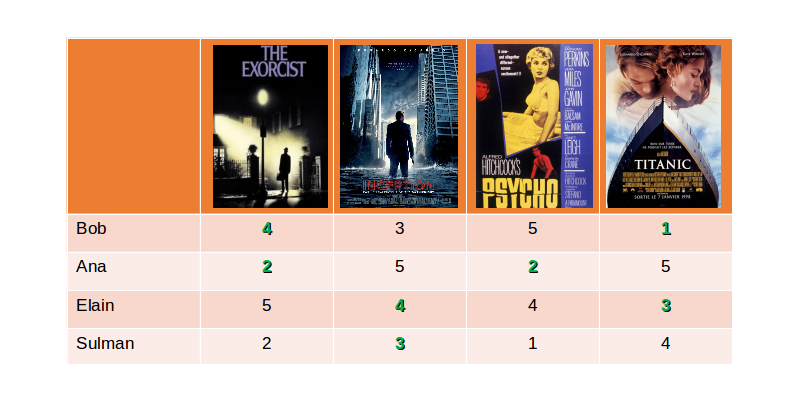
\includegraphics[scale=0.6]{images/task2.png}
\caption{电影评分预测任务样例2}
\label{fig:task2}
\end{figure}

假设我们已经构建好模型,并成功预测出如图\ref{fig:task2}所示的评分结果,
那么我们可以根据用户Bob可能给电影《The Exorcist》评价$5$分而给电影《Titanic》评价$1$分的预测评分结果,
来将电影《The Exorcist》推荐给用户Bob。

\section{基本假设}
协同过滤算法的基本假设是,被相同用户偏爱的物品具有相似的兴趣分布,
或者喜欢相同物品的用户拥有相似的兴趣分布。然而在现实的环境中,
由于用户的兴趣会随着时间发生变化(兴趣漂移),这样的假设并不总是成立。
但是从另外一个角度而言,对于一个给定的用户,在一个给定的时间段内,
该用户的兴趣分布往往是稳定的,不会发生剧烈的变化。

\begin{figure}[htbp]
\centering
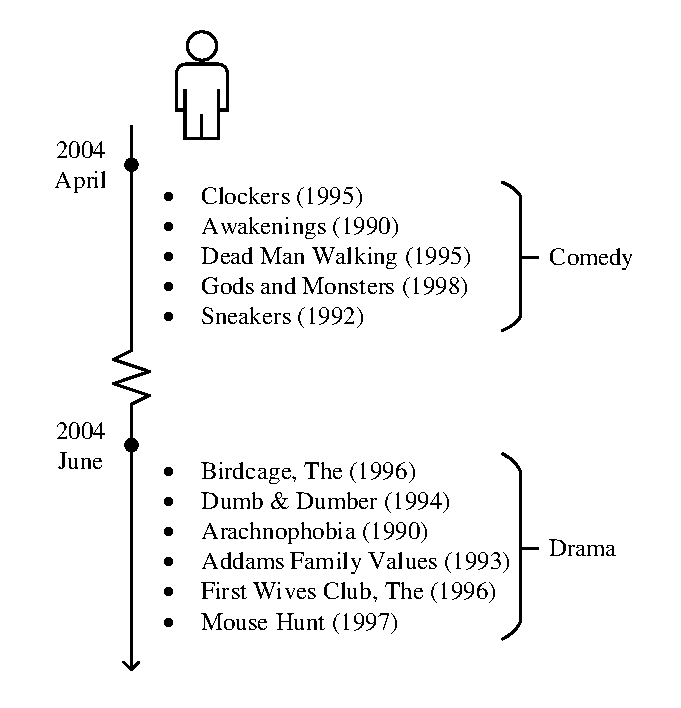
\includegraphics[scale=0.75]{images/example.pdf}
\caption{数据集MovieLens-1M中ID号为$5988$的用户的观影时间线}
\label{fig:example}
\end{figure}

例如,对于著名推荐系统数据集MovieLens-1M中一名ID号为$5988$的用户,
我们将他的电影评分数据按照时间进行排序,构成了图\ref{fig:example}所展示的观影时间线。
从图中我们可以观察得到,该用户在2004年四月份的时候热衷于观看喜剧类电影,
然后在2004年六月份开始转为喜爱观看戏剧类电影。

为了描述这种现象,本文提出了两个定义:长时间兴趣分布和短时间兴趣分布,
它们的具体描述如下:

\begin{enumerate}
\item \textbf{长时间兴趣分布}反映了用户在整个时间区间上的兴趣分布,
它体现在用户在整个时间区间上所有喜爱和讨厌的物品的整体集成上。
\item \textbf{短时间兴趣分布}反映了用户在某一固定时间子区间上的兴趣分布,
它体现在用户在这个固定时间子区间上所有喜爱和讨厌的物体的整体集成上。
\end{enumerate}

从两者的定义可以看出,一个用户可以拥有一个长时间兴趣分布和若干短时间兴趣分布。
在图\ref{fig:example}的例子中,ID号为$5988$的用户的长时间兴趣分布就是
既喜爱观看喜剧类电影又喜爱观看戏剧类电影,同时该用户又拥有两个短时间兴趣,
一个是四月份的喜爱观看喜剧类电影,另外一个是六月份喜爱观看戏剧类电影。

在传统协同过滤算法中,模型只考虑用户的长时间兴趣分布,
即这两个不同种类的电影由于同时被当前用户所喜爱而被同等对待处理,
但实际上它们的类型是不同的。
本文研究的起点就是研究如何更加合理地利用短时间兴趣分布来提高推荐系统的推荐性能。

下面我们将说明我们提出的两个新的假设,紧接着,我们介绍基于新假设的长短期兴趣模型,
最后我们利用长短期兴趣模型获得的用户特征和物品特征生成最终的评分结果。

\section{两个新的假设}
用户的长时间兴趣分布体现在整个时间区间中交互过的物品上,
短时间兴趣分布体现在若干时间子区间中交互过的物品上,
并且随着时间的推移不断发生变化,为了体现短时间兴趣分布的特点,
本文提出了两个新的假设,如下所示:

\begin{enumerate}
\item 对于同一个长时间兴趣分布中的若干短时间兴趣分布,
处于相同短时间兴趣分布中的物品之间的相似度大于
处于不同短时间兴趣分布中的物品之间的相似度。
\item 对于不同的长时间兴趣分布中的若干短时间兴趣分布,
物品同时出现在同一个短时间兴趣分布的次数和他们之间的相似度呈正相关关系,
即出现次数越多,物品之间的相似度越高,反之,出现次数越少,
物品之间的相似度越低。
\end{enumerate}

\begin{figure}[htbp]
\centering
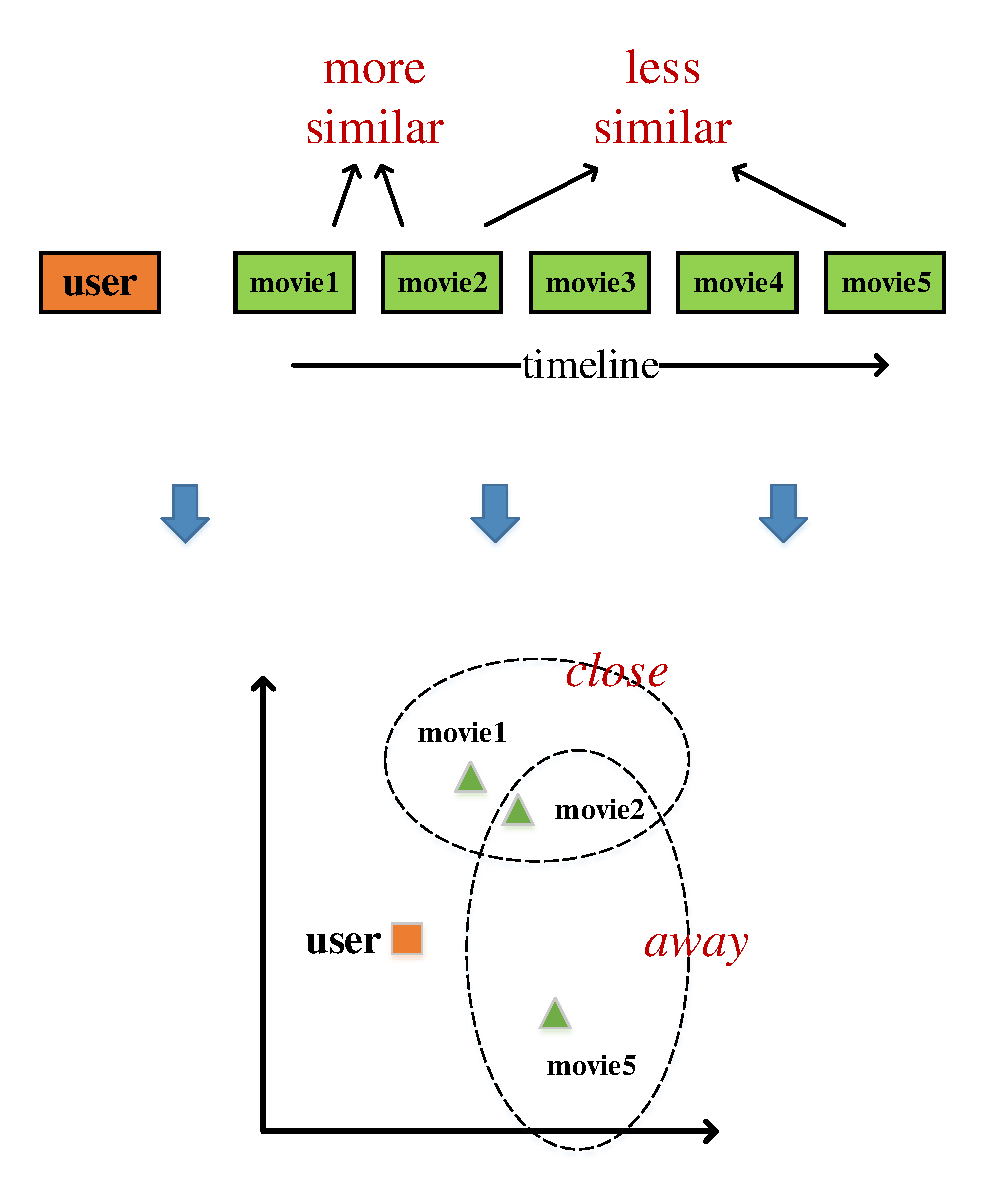
\includegraphics[scale=0.5]{images/embedding.pdf}
\caption{物品之间的相似度在低秩嵌入空间中的表现}
\label{fig:embedding}
\end{figure}

以图\ref{fig:embedding}为例,在图的上半部分,
用户$user$观看了$item1$,$item2$,$item3$,$item4$和$item5$五部电影,
我们将其按照时间进行排序,形成用户的观影时间线。
如果假设短时间的时间窗口长度为$2$,那么该用户就拥有$4$个短时间兴趣模型,
<$item1$,$item2$>,<$item2$,$item3$>,<$item3$,$item4$>和
<$item4$,$item5$>。
$item2$和$item1$处于同一个短时间兴趣分布,
$item2$和$item5$处于不同的短时间兴趣分布,
根据我们的第一个假设,
那么$item2$和$item1$的相似度应该大于$item2$和$item5$的相似度。
在图的下半部分,我们给出了在低秩嵌入空间中三者的空间位置,
通过向量之间的距离关系对应不同电影之间的相似度,
可以看到$item2$和$item1$的嵌入向量之间的距离小于
$item2$和$item5$的嵌入向量之间的距离。

\section{长短期兴趣模型}
自然语言处理Paragraph2Vec算法\parencite{le2014distributed}利用语句模型中
的单词顺序学习出有效的嵌入向量表示,在情感分类和信息检索任务上取得了较优的实验效果。
受到该算法的启发,本文提出了一个长短期兴趣模型(Long-Short Interest Model, LSIM),
基于提出的两个新的假设,从观影时间线中提取序列信息,
学习出更好的用户嵌入向量表示和物品嵌入向量表示。

\begin{figure}[htbp]
\centering
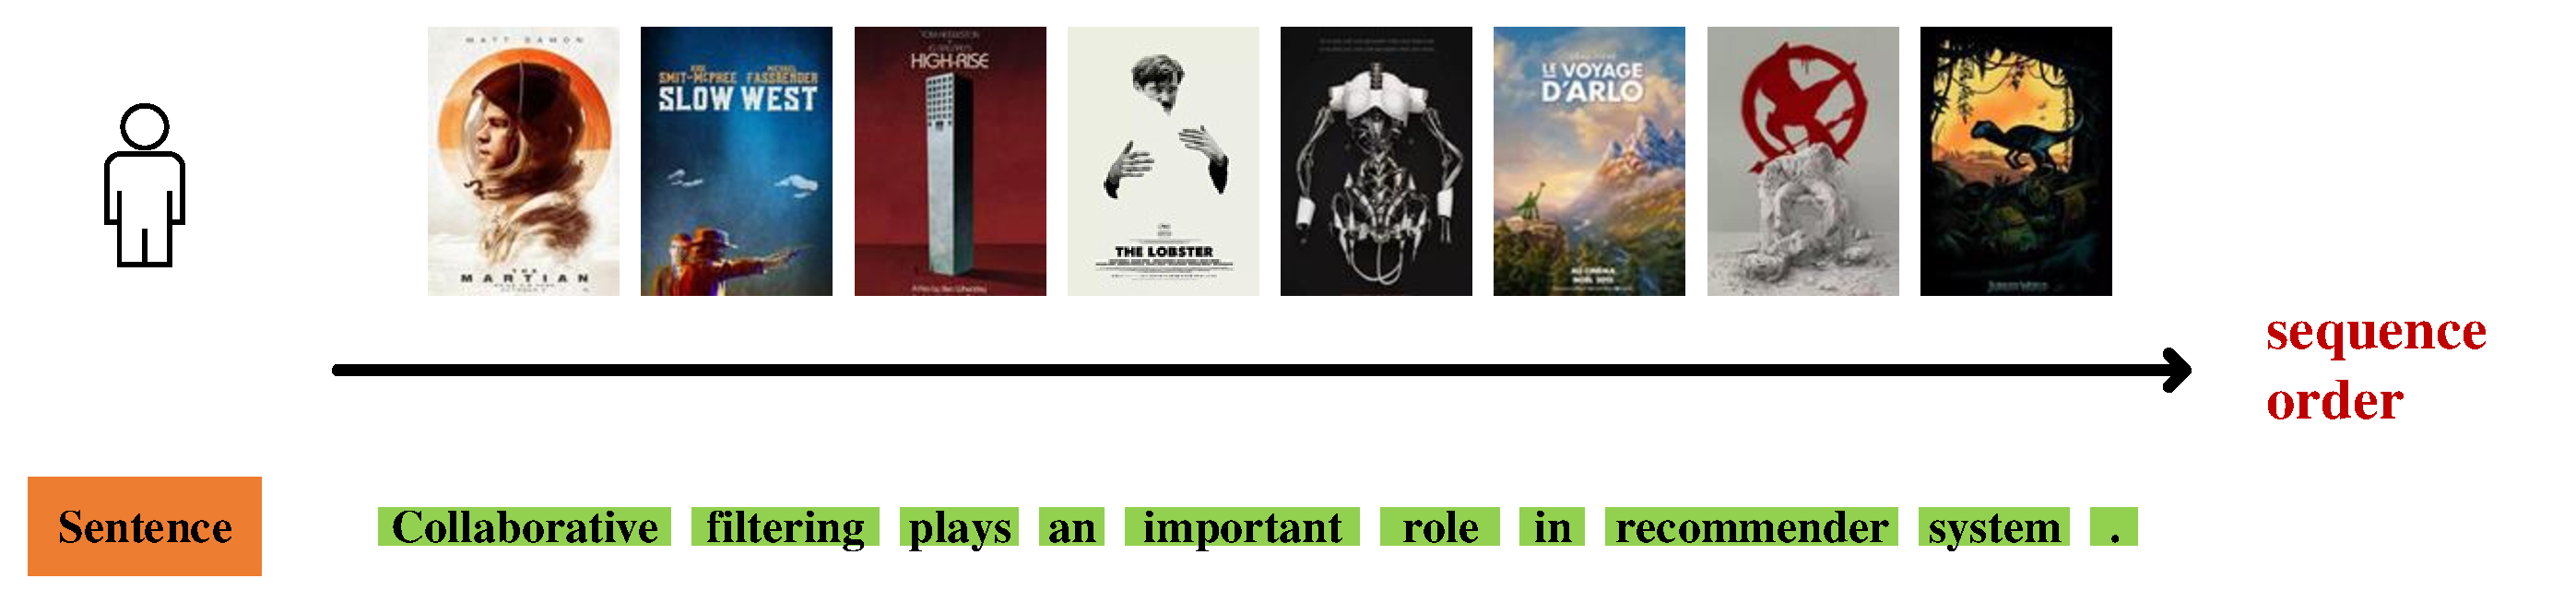
\includegraphics[scale=0.3]{images/example2.pdf}
\caption{Paragraph2vec learns vector representations of sentences and words
    based on the word order
    while LSIM extracts sequential features of users and items
    based on the rating order.
}
\label{fig:example2}
\end{figure}

如图\ref{fig:example2}所示,推荐算法中的用户类似于自然语言处理中的语句,
它们的共同点是都包含一个符合特定顺序关系的序列,
推荐短发中的物品类似于自然语言处理中的语句中的词语,
它们的共同点是都符合相对距离越近,相似程序越高的特点。

\begin{figure}[htbp]
    \centering
    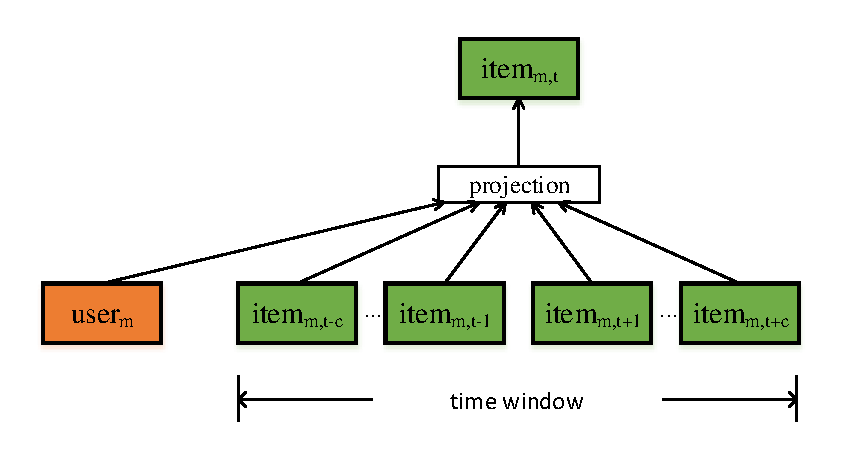
\includegraphics[scale=0.6]{images/doc2vec.pdf}
    \caption{Embedding Model for Extracting Interest Similarity from Users and Items}
    \label{fig:doc2vec}
\end{figure}

通过将用户作为一个全局的上下文信息,长短期兴趣同时学习出用户嵌入向量和物品嵌入向量,
整个模型的结构如图\ref{fig:doc2vec}所示。

假设推荐系统中存在$N$个用户$x_i(i \in 1,2,...,N)$以及$M$部电影$y_j(j \in 1,2,...,M)$
\footnote{我们使用符号$x和$y$代替经典的$u和$v$以避免符号$v$和向量符号$\mathbf{v}$在阅读上的误解},
每一个用户都拥有一个观影时间线$T_i(i \in 1,2,...,N)$,
包含了按照时间排序的若干电影信息$y_{i_1}$, $y_{i_2}$, ..., $y_{i_{L_i}}$,
其中$L_i$代表用户$x_i$观影时间线上电影的数量,其数值远远小于电影数量$M$。

为了建模长时间兴趣分布,我们考虑将整个观影时间线的电影作为上下文生成当前用户,
即
\begin{equation}
p(x_i | y_{i_1}, y_{i_2}, ..., y_{i_{L_i}})
\end{equation}

为了建模短时间兴趣分布,对于用户观影时间线上面的每一部电影,
我们考虑将用户和当前短时间窗口中的其他电影作为上下文来生成目标电影,
即
\begin{equation}
\sum_{j=1}^{L_i} p(y_{i_j} | y_{i_{j-c}} : y_{i_{j+c}}, x_i)
\end{equation}
其中$c$是时间窗口大小,$y_{i_{j-c}} : y_{i_{j+c}}$代表不包含
$y_{i_j}$项的序列$y_{i_{j-c}}, y_{i_{j-c+1}}, ..., y_{i_{j+c}}$。

所以更加正式地说,长短期兴趣模型的目标是最大化所有用户的
观影时间线$T_i(i \in 1,2,...,N)$的极大似然概率,
即
\begin{equation}
\sum_{i=1}^{N} \bigg( p(x_i | y_{i_1}, y_{i_2}, ..., y_{i_{L_i}}) +
\sum_{j=1}^{L_i} p(y_{i_j} | y_{i_{j-c}} : y_{i_{j+c}}, x_i) \bigg)
\end{equation}

其中$p(x_i | y_{i_1}, y_{i_2}, ..., y_{i_{L_i}})$是基于观看过的电影
生成$u_i$的长期兴趣的概率,这是一种典型的预测问题,我们可以使用多分类的方法解决,
例如Softmax,因此我们得到

\begin{equation}
p(x_i | y_{i_1}, y_{i_2}, ..., y_{i_{L_i}}) =
\frac
{
    exp ( \overline{\mathbf{v}}_{1}^{\mathrm{T}} \mathbf{v}_{x_i}^{'} )
}
{
    \sum_{x^{'}} exp ( \overline{\mathbf{v}}_{1}^{\mathrm{T}} \mathbf{v}_{x^{'}}^{'} )
}
\end{equation}

其中$\mathbf{v}_{x_i}^{'}$是用户$x_i$的输出向量表示,
$\overline{\mathbf{v}}_{1}$代表用户$x_i$的观影时间线上的所有电影的输入向量的平均值,
即
\begin{equation}
\overline{\mathbf{v}}_{1} = \frac{\sum_{j=1}^{T_i} \mathbf{v}_{y_{i_j}}}{T_i}
\end{equation}

而$p(y_{i_j} | y_{i_{j-c}} : y_{i_{j+c}}, x_i)$是使用用户长期兴趣和
同一个时间窗口内的其他电影生成$y_{i_j}$的概率,这也是一个多分类任务,
同样地,我们使用Softmax进行求解,即
\begin{equation}
p(y_{i_j} | y_{i_{j-c}} : y_{i_{j+c}}, x_i) =
\frac
{
    exp( \overline{\mathbf{v}}_{2}^{\mathrm{T}} \mathbf{v}_{y_{i_j}}^{'} )
}
{
    \sum_{y^{'}} exp( \overline{\mathbf{v}}_{2}^{\mathrm{T}} \mathbf{v}_{y^{'}}^{'} )
}
\end{equation}

其中$\mathbf{v}_{y_{i_j}}^{'}$代表电影$y_{i_j}$的输出向量表示,
$x_i$表示用户的长期兴趣向量表示
而$\overline{\mathbf{v}}_{2}$是同一个短期兴趣窗口内其他电影的向量表示的平均值,
即
\begin{equation}
\overline{\mathbf{v}}_{2} = \frac{
    \mathbf{v}_{x_i} + 
    \sum_{-c \leq k \leq c, k \not= 0}{\mathbf{v}_{y_{i_{j+k}}}}
}{2c+1}
\end{equation}

我们使用随机梯度下降(Stochastic Gradient Descent, SGD)对优化目标进行迭代求解,
同时层次Softmax(Hierarchical Softmax)和负采样(Negative Sampling)是
两个常见的计算加速算法,在本文中,我们使用负采样的方法进行计算加速。

\section{电影评分生成}
基于特征的协同过滤 \parencite{chen2011feature} 是协同过滤的一个变种,
和传统的矩阵分解不同的是,它允许我们在创建分解模型的同时利用诸多辅助信息,
例如用户画像,物品属性,好友关系和时间动态等等。

协同过滤中的特征一般可以分成两类:用户特征和物品特征,
我们使用$\mathbf{u}_i \in \mathbb{R}^{n}$代表用户特征,
$\mathbf{v}_j \in \mathbb{R}^{m}$代表物品特征,
那么预测评分数值$\hat{r}$ 的公式为

\begin{equation}
\hat{r}_{ij} = \sum_{k=1}^{n} \alpha_k \mathbf{u}_{ik} + \sum_{k=1}^{m} \beta_k \mathbf{v}_{jk} +
\left( \sum_{k=1}^{n} \mathbf{u}_{ik} \mathbf{p}_k \right) ^ \mathrm{T}
\left( \sum_{k=1}^{m} \mathbf{v}_{jk} \mathbf{q}_k \right)
\end{equation}

其中$\alpha$和$\beta$分别控制着用户特征和物品特征的影响程度
$\mathbf{p}_{k} \in \mathbb{R}^K$和$\mathbf{q}_{k} \in \mathbb{R}^K$
是$K$维的和每一个特征相关的隐向量因子。
如果我们使用独热向量(One-Hot Representation)来表示用户和物品,即
\begin{equation}
\mathbf{u}_{ik} =
\left\{
\begin{aligned}
1, &k = i \\
0, &k \not= i
\end{aligned}
\right. \\ , 
\mathbf{v}_{jk} =
\left\{
\begin{aligned}
1, &k = j \\
0, &k \not= j
\end{aligned}
\right. \\
\end{equation}

那么上文中的评分预测公式就会退化为基本的矩阵分解算法,
即
\begin{equation}
\hat{r}_{ij} = \alpha_i + \beta_j + \mathbf{p}_i ^ \mathrm{T} \mathbf{q}_j
\end{equation}

其中$\alpha$和$\beta$分别代表用户偏移和物品偏移,
而$\mathbf{p}_i$和$\mathbf{q}_j$分别代表用户$\mathbf{u}_i$和物品$\mathbf{v}_j$
对应的隐向量因子。


在本文的工作中,我们使用长短期兴趣模型中学习出来的用户表示和物品作为一种辅助信息。
因此,我们定义$\tilde{\mathbf{u}}_i$代表学习出来的用户表示,
$\tilde{\mathbf{v}}_j$代表学习出来的物品表示。
然后,我们通过组合学习出的用户物品表示和经典的独热表示得到新的特征组合,即

\begin{equation}
\mathbf{u}_{i} = \{ \mathbf{u}_{i} , \tilde{\mathbf{u}}_i \} , 
\mathbf{v}_{j} = \{ \mathbf{v}_{j} , \tilde{\mathbf{v}}_j \}
\end{equation}

因此评分预测的公式将会变为

\begin{equation}
\begin{aligned}
\hat{r}_{ij} =
&\sum_{k=1}^{N+D} \alpha_k \{ \mathbf{u}_i , \tilde{\mathbf{u}}_i \}_k +
\sum_{k=1}^{M+D} \beta_k  \{ \mathbf{v}_j , \tilde{\mathbf{v}}_j \}_k + 
&\left( \sum_{k=1}^{N+D} \{ \mathbf{u}_i , \tilde{\mathbf{u}}_i \}_k \mathbf{p}_k \right) ^ \mathrm{T}
\left( \sum_{k=1}^{M+D} \{ \mathbf{v}_j , \tilde{\mathbf{v}}_j \}_k \mathbf{q}_k \right)
\end{aligned}
\end{equation}

其中$N$是推荐系统中的用户的数量,$M$是推荐系统中物品的数量,
$D$本文提出的长短期兴趣模型中学习出来的用户特征和物品特征的维度,
$\mathbf{p}_{k} \in \mathbb{R}^K$和$\mathbf{q}_{k} \in \mathbb{R}^K$
是$K$关联到每个特征的隐向量因子的维度。


